\documentclass[crop,tikz]{standalone}
\usetikzlibrary{backgrounds}
\colorlet{blue}{cyan}
\tikzset{
  inverted/.style = {
    color=white,
    background rectangle/.style={fill},
    show background rectangle
  }
}

\usepackage{amsmath}
\tikzset{>=latex}
\colorlet{green}{green}
\newcommand{\F}{\vec{F}}
\newcommand{\ort}{\vec{r}}
\newcommand{\vs}{\vec{s}}
\newcommand{\dvr}{\text{d}\ort}

\begin{document}
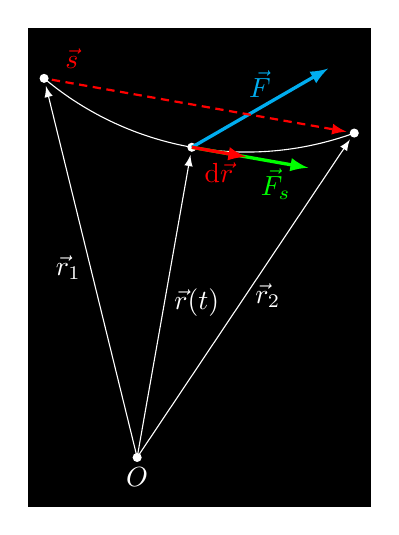
\begin{tikzpicture}[inverted,inverted]
  \coordinate (a) at (230:4);
  \coordinate (c) at (260:4);
  \coordinate (o) at (260:8);
  \draw (a) arc (230:290:4) coordinate (e);
  \draw[fill] (a) circle (0.05);
  \draw[fill] (e) circle (0.05);
  \draw[fill] (c) circle (0.05);
  \draw[fill] (o) circle (0.05) node[below] {$O$};
  \draw[->,shorten >= 1mm] (o) -- node[left]  {$\ort_1$} (a);
  \draw[->,shorten >= 1mm] (o) -- node[right] {$\ort(t)$} (c);
  \draw[->,shorten >= 1mm] (o) -- node[right] {$\ort_2$} (e);
  \draw[->,blue,very thick]  (c) -- node[above] {$\F$} +(30:2);
  \draw[->,green,very thick] (c) -- node[below right] {$\F_s$} +(350:1.5);
  \draw[->,red ,very thick]  (c) -- node[below] {$\dvr$} +(350:0.7);
  \draw[->,red,densely dashed,thick,shorten <= 1mm,shorten >= 1mm] (a) -- (e);
  \node[red,above,xshift=1em] at (a) {$\vs$};
\end{tikzpicture}
\end{document}
